\documentclass{sigchi}

% Use this command to override the default ACM copyright statement
% (e.g. for preprints).  Consult the conference website for the
% camera-ready copyright statement.


%% EXAMPLE BEGIN -- HOW TO OVERRIDE THE DEFAULT COPYRIGHT STRIP -- (July 22, 2013 - Paul Baumann)
% \toappear{Permission to make digital or hard copies of all or part of this work for personal or classroom use is      granted without fee provided that copies are not made or distributed for profit or commercial advantage and that copies bear this notice and the full citation on the first page. Copyrights for components of this work owned by others than ACM must be honored. Abstracting with credit is permitted. To copy otherwise, or republish, to post on servers or to redistribute to lists, requires prior specific permission and/or a fee. Request permissions from permissions@acm.org. \\
% {\emph{CHI'14}}, April 26--May 1, 2014, Toronto, Canada. \\
% Copyright \copyright~2014 ACM ISBN/14/04...\$15.00. \\
% DOI string from ACM form confirmation}
%% EXAMPLE END -- HOW TO OVERRIDE THE DEFAULT COPYRIGHT STRIP -- (July 22, 2013 - Paul Baumann)


% Arabic page numbers for submission.  Remove this line to eliminate
% page numbers for the camera ready copy 

%\pagenumbering{arabic}

% Load basic packages
\usepackage{balance}  % to better equalize the last page
\usepackage{graphics} % for EPS, load graphicx instead 
%\usepackage[T1]{fontenc}
\usepackage{txfonts}
\usepackage{times}    % comment if you want LaTeX's default font
\usepackage[pdftex]{hyperref}
% \usepackage{url}      % llt: nicely formatted URLs
\usepackage{color}
\usepackage{textcomp}
\usepackage{booktabs}
\usepackage{ccicons}
\usepackage{todonotes}

% llt: Define a global style for URLs, rather that the default one
\makeatletter
\def\url@leostyle{%
  \@ifundefined{selectfont}{\def\UrlFont{\sf}}{\def\UrlFont{\small\bf\ttfamily}}}
\makeatother
\urlstyle{leo}

% To make various LaTeX processors do the right thing with page size.
\def\pprw{8.5in}
\def\pprh{11in}
\special{papersize=\pprw,\pprh}
\setlength{\paperwidth}{\pprw}
\setlength{\paperheight}{\pprh}
\setlength{\pdfpagewidth}{\pprw}
\setlength{\pdfpageheight}{\pprh}

% Make sure hyperref comes last of your loaded packages, to give it a
% fighting chance of not being over-written, since its job is to
% redefine many LaTeX commands.
\definecolor{linkColor}{RGB}{6,125,233}
\hypersetup{%
  pdftitle={SIGCHI Conference Proceedings Format},
  pdfauthor={LaTeX},
  pdfkeywords={SIGCHI, proceedings, archival format},
  bookmarksnumbered,
  pdfstartview={FitH},
  colorlinks,
  citecolor=black,
  filecolor=black,
  linkcolor=black,
  urlcolor=linkColor,
  breaklinks=true,
}

% create a shortcut to typeset table headings
% \newcommand\tabhead[1]{\small\textbf{#1}}

% End of preamble. Here it comes the document.
\begin{document}

\newcommand{\getTitleName}{HandTie}

\title{\getTitleName\ : Exploring Gestural Interface on Back of the Hand}

\numberofauthors{3}
\author{%
  \alignauthor{1st Author Name\\
    \affaddr{Affiliation}\\
    \affaddr{City, Country}\\
    \email{e-mail address}}\\
  \alignauthor{2nd Author Name\\
    \affaddr{Affiliation}\\
    \affaddr{City, Country}\\
    \email{e-mail address}}\\
  \alignauthor{3rd Author Name\\
    \affaddr{Affiliation}\\
    \affaddr{City, Country}\\
    \email{e-mail address}}\\
}

\maketitle

\begin{abstract}

\end{abstract}

\keywords{Gesture recognition; wearable interface; strain gauge; machine learning; gestural interaction }

\category{H.5.m.}{Information Interfaces and Presentation
  (e.g. HCI)}{Miscellaneous} \category{See
  \url{http://acm.org/about/class/1998/} for the full list of ACM
  classifiers. This section is required.}{}{}

%直接用target sensing的位置去分類,分三類,手指、手腕、手臂
%可以說手指偵測就得直接裝在手指上,不然就是CV的太耗電問題。可是戴在手腕上和戴在手臂上會不準,小動作偵測不到。


\section{Introduction}
Hand gestures have become popular and powerful means of human computer interface nowadays.
Gesture interaction can serve as an effective and natural modality to communication between humans and computers.
However, the key problem in gesture interaction is how to make hand gestures understood by the computer. %保留這句原意,但幫修改句構(因抄來的,前兩句不用)

% Gesture interaction offers more effective expression and complements verbal communication in a conversation.
%Gesture interaction can serve as a complementary modality to communication to express ones ideas.

% According to the sensor's target position on the hand, there are many on-body gestural interfaces which can mainly be classified into two categories:(1) interfaces based on the finger's measurement , (2) interfaces based on wrist or arm measurement.
%see figureX

Based on the source of the sensor's input signal, numerous on-body gestural interfaces can mainly be classified into three categories: (1) interfaces measuring physical movement directly from fingers, (2) interfaces measuring physical properties from wrist, (3) interfaces measuring physical properties from arm. See \autoref{fig:HandTarget}.

Finger-based gestural interfaces are devices mostly in a glove-like form where sensors are placed directly on the joints of fingers \cite{4539650}. Gestures performed by users are accurately captured through such devices. Nonetheless, data gloves or mechanical structures worn on the hand cause discomfort and obstruct agility of fingers.
Another approach utilizing vision-based techniques resolve the disadvantages of glove-like devices. Despite the fact that a vision-based device is worn on the wrist \cite{Kim:2012:DFI:2380116.2380139}, it is still classified as a finger-based gestural interface because its input signal source also originates directly from finger movements. A vision-based approach also results in high accuracy of gesture recognition or hand tracking. Cameras suffer from line-of-sight occlusions and have large power consumption and heavy computation requirements limiting the battery life of such devices.

\begin{figure}
  \begin{center}
  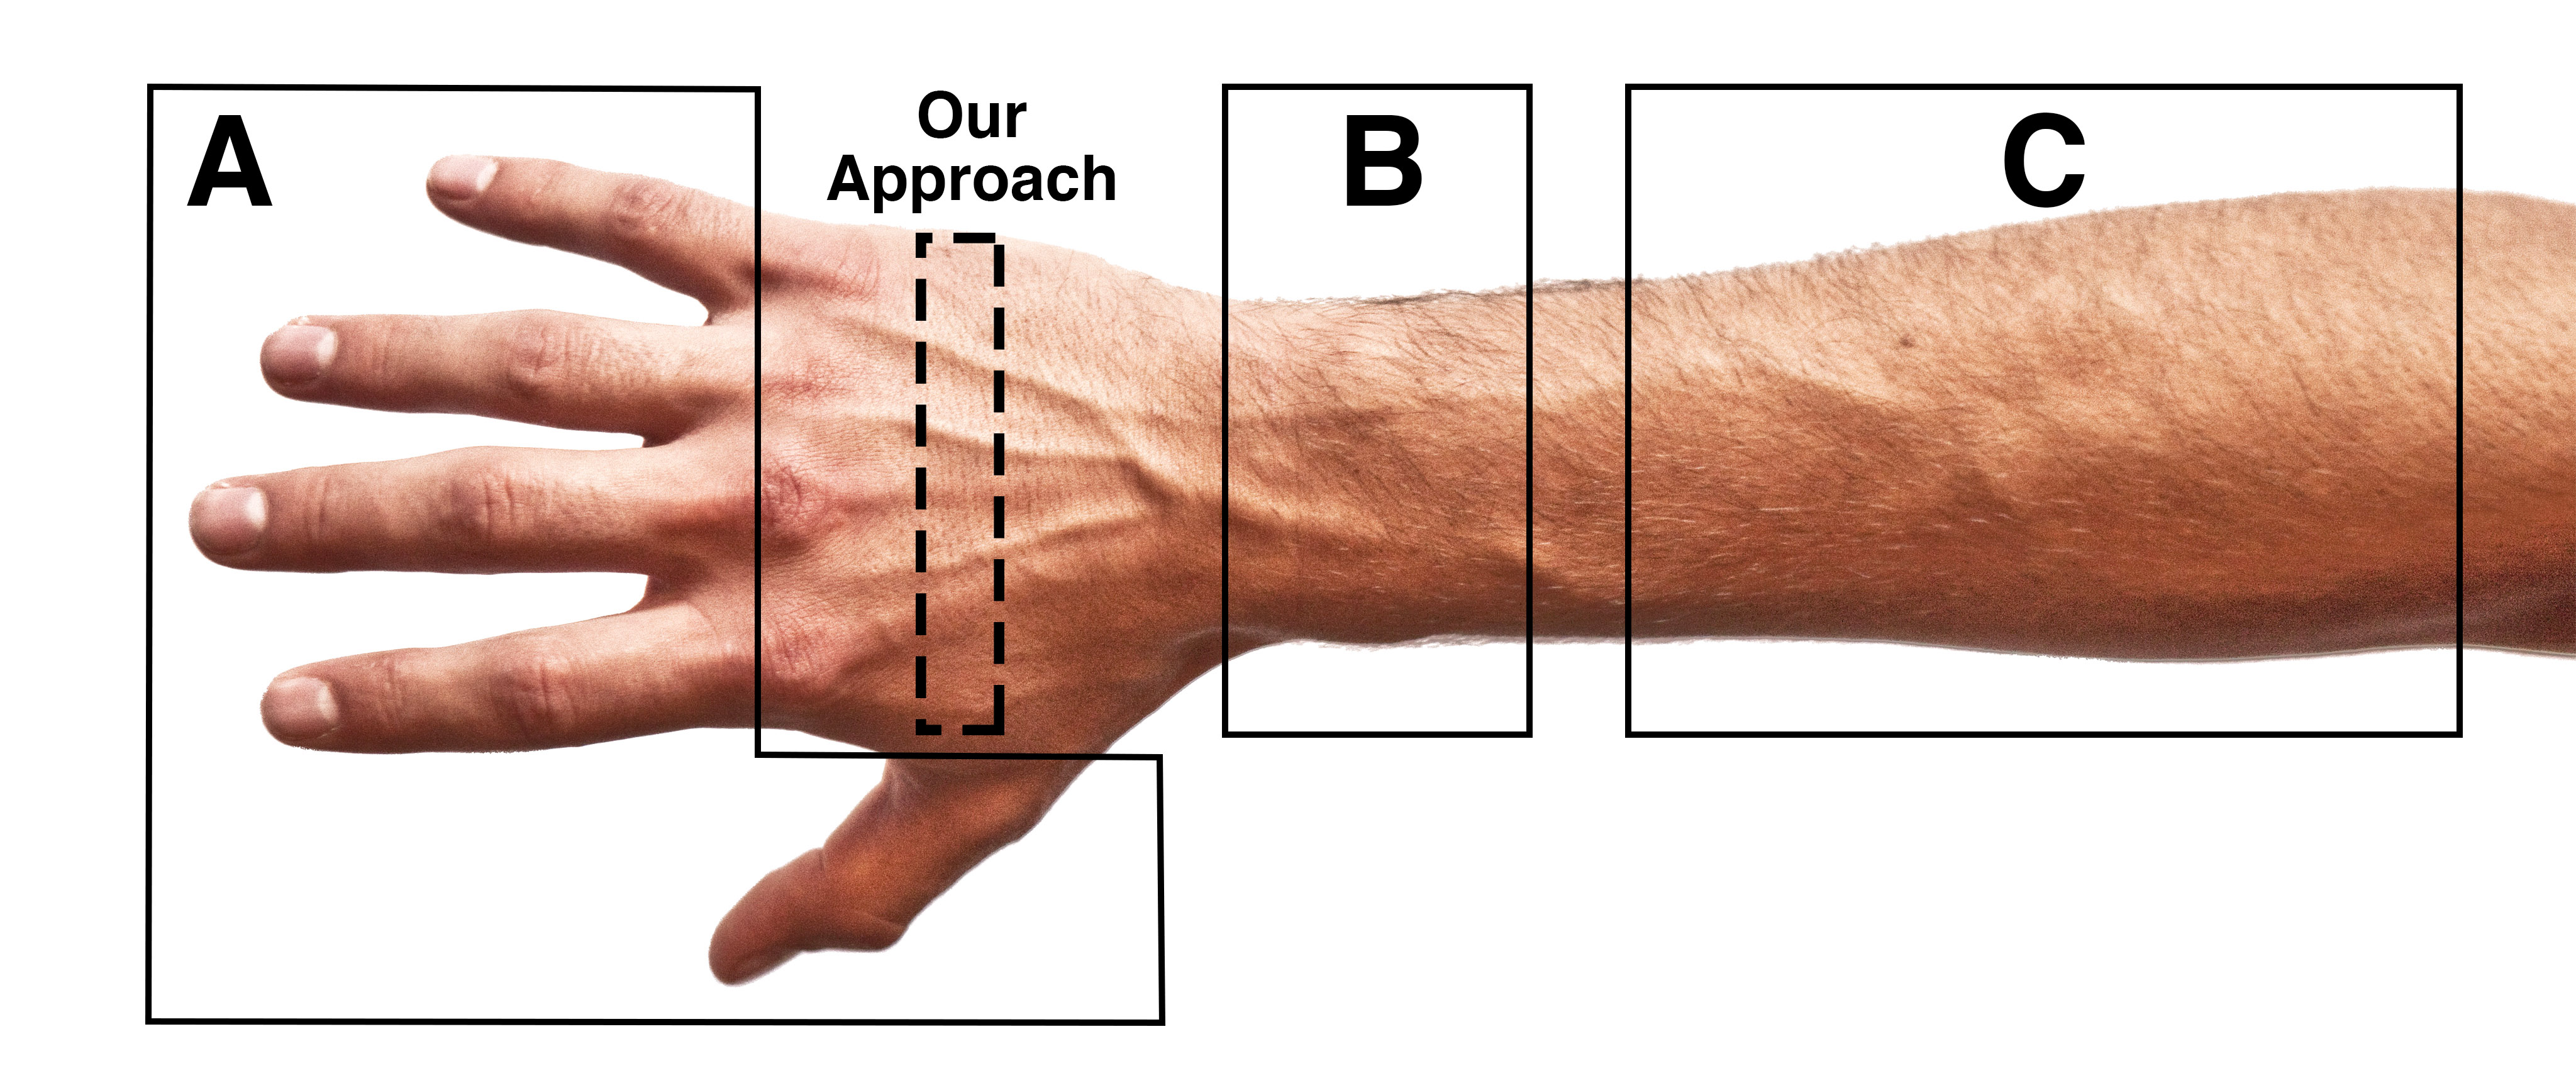
\includegraphics[width=1\columnwidth]{figures/HandTarget.png}
  \caption{The three common body parts as sources of a sensor's input signal for a gestural interface include (A) the fingers, (B) the wrist, and (C) the arm.}
  \label{fig:HandTarget}
  \end{center}
\end{figure}

Wrist-based gestural interfaces are much rare compared to finger-based gestural interfaces and arm-based gestural interfaces. Wrist-worn wearable devices are the most friendly and acceptable interfaces. However, based on previous works adopting capacitive sensing technique \cite{Rekimoto:2001:GGU:580581.856565}, vision-based technique \cite{Dementyev:2014:WLG:2642918.2647396}, and force-sensitive sensing approach \cite{Fukui:2011:HSC:2030112.2030154}, changes in physical properties of the tendons on the wrist barely deliver distinguishable signals among finger gestures bringing about a very small number of gestures supported and low accuracy of recognition.

Arm-based gestural interfaces employ electromyographical sensing technique where a device is placed right on the arm \cite{Myo} or below the elbow \cite{Saponas:2009:EAI:1622176.1622208} to measure electrical potential differences between pairs of electrodes. Such interfaces usually support gestures involving full hand movements (e.g., clenched fist and splayed fingers) or arm movements at a fairly high accuracy rate. However, finer gestures involving single finger movements are not discernible to such devices.

Among the previous works, \autoref{fig:HandTarget} shows the three common body parts as the input signal sources of various sensing techniques. It is concluded that in general the closer the source is to the fingers, the greater the accuracy rate of finer gesture recognition is obtained, and vice versa. For practical usage, a tradeoff (e.g., measurement accuracy versus comfort, measurement accuracy versus expense, computational overhead versus comfort) must be considered among the countless related works. In this work, we manage to combine the beneficial characteristics of these works through a different approach by exploring another potential body part as an input source other than those listed in \autoref{fig:HandTarget}. That is the back of hand.

% To gather high accuracy information of hand movements, one approach is to instrument the hand with a glove-based gestural interface which is equipped with a number of sensors which provide information about hand position, orientation, and bending angles of fingers. Although these data glove-like systems are different in sensor technologies, locations, and mounting, they all share three basic design concepts: they measure finger joint bending, use a cloth for supporting sensors, and are usually meant to be general-purpose devices \cite{4539650}. 

%我覺得需要利用citation的方式明確舉例work
% Although most of these finger-based systems provide high accuracy, high reliability, and high capability in measuring the degrees-of-freedom (DoF) of human hands, they suffered from several drawbacks. Major limitations originated from the cloth support, which acted as a constraint on the user’s hand. For instance, they have to be worn on the fingers to measure the flex of the fingers. Such complications may reduce dexterity of the hand. Additionally, these systems can be complex, expensive, and cumbersome for users.
% The constraints of traditional glove-based systems make them poor candidates for use in mobile applications. 

%一樣,需要利用citation的方式明確舉例work
%On the other hand, From another approach
% In the past couple of years, a number of gestural interfaces for alphanumerical character entry in wearable and portable computers have been proposed. Since these devices are usually worn on the wrist or arm, they introduce a unique opportunity to understand user’s arm, hand and possibly finger movements. While all these devices stand out for their originality and overcome some of the limitations of the data glove-like devices(e.g., most have no cloth), they have individual limitations. Additionally, they were designed for specific applications rather than for general purpose. Although they may be suitable for gesture-based applications outside the wearable and portable computer area due to their accessibility, they appear to be unsuitable for applications that require high measurement performance and the diversity of gesture types.

% In the past, when we have to determine which gestural interface to be used, there is a tradeoff between the accuracy of measurements and portability. Apparently, there are some new techniques usually act differently between the glove-based systems and gestural interfaces in wearable and portable computers and even combine the beneficial characteristics of both systems.

%是否需要強調:「我們試圖用最小的覆蓋面積,達到手背的最大使用」
% \getTitleName\ is an elegant and powerful gestural interface that shared the beneficial characteristics of BOTH systems. both???你的系統有哪些?這樣有點ambiguous!
% 以上三種分類,誒,怎麼寫不出來了,剛剛不是講話很大聲的嗎XDDD

% 我們認為研究將手背作為感測目標是極具吸引人的
% attractive location

% 當裝置感測目標位於手背時,這樣的裝置具有以下四個特色:

% First,不干擾裝置:當手指、手腕、手臂在空間中與環境互動時,通常會干擾裝置感測,如:握持物體遮擋camera,或手腕關節活動干擾手腕裝置

% Second,不受裝置干擾:手背屬於平坦並且日常中不常使用的地方,可以避免穿戴者在進行手部關節運動時受到裝置干擾,如:手指被手套包覆除了不靈活也degrade tactile sensation,或者將裝置穿戴於手腕,影響手腕關節活動(wristflex)。

% Third,精準:提供接近於手指作為感測目標手勢辨識的精準度

% Fourth,不受外部環境影響:一般以vision或聲音為基礎的gestual interface,容易受到外部光源或聲音的干擾

%  \getTitleName\ is an elegant and powerful gestural interface that 將感測目標面對手背。
 
%  此系統的prototype藉由在人工皮載體上放置感應靈敏之應變感應器陣列,可以細微的觀測手背變形程度變化。
 
%  我們用這樣的裝置,來探索在手背這樣寬廣且平坦的地方,哪裡最適合放置感應裝置。

\getTitleName\ is an elegant and powerful gestural interface that falls into a new category of input signal source as the back of hand. The prototype consisting of a artificial skin where an array of strain sensors are attached measures any physical changes on the back of hand.

There are also several reasons to choose the back of hand as the source of sensor's input signal:

% There are also several reasons to choose the back of hand as the source of sensor's input signal:(1) , (2), (3) measurement accuracy.

%First, strain sensors placed on the back of hand are less prone to false detection and ____ caused by the user's daily-life behaviour.
% First, joint movement of body parts such as fingers, wrist, and arm interacting with tangible objects usually interfere with its sensing operation.
First, interactions with tangible objects often interfere with the sensing operation.
For instance, a grasp of an object blocks the camera worn on the wrist capturing finger movements.
Sensors attached to joints could also cause false positives by a joint movement.
For another instance, physical wrist movements can cause unintended results to the wrist-based gestural input device.
Sensing physical changes on the back of hand are not subject to such technical limitations.
Second, the back of hand without joints is a surface with less curvature and has less chance of physical contact with other objects under most circumstances. Moreover, unlike fingers and palms, the back of hand is not a body part effectively for productivity and interactions with tangible objects. Hence, strain sensors on the back of hand do not reduce dexterity of the hands and contribute less discomfort and less degradation of tactile sensation compared to that of glove-like devices.
Third, high measurement accuracy is obtained due to its nearby location to the fingers.
% Fourth, external noises such as light and sound do not interfere such device.
 
% (e.g., high measurement performance, high reliability, versatile gesture types, portability).

%Traditional glove-based systems cover most of the fingers to measure the flex of the fingers; gestural interfaces in wearable and portable computers are usually worn on the wrist or arm.
% We explore the back of hand to be an attractive location for an alternative gestural interface that simply affixes on the users' back of the hand.

In addition to this device that can detect subtle finger movements from the deformation distribution on the back of the hand, the contributions of this work also include an exploration of the influence of various gestures on it and then address the optimal sensor placement,
associated hardware and software design spaces,
an evaluation of the levels of recognition accuracy and performance,
and a set of applications and broader interactions with the different usage scenarios that are enabled by \getTitleName.

%請把上一段落變成列點式:
% \begin{itemize}
% \item We ... exploration of the influence of various gestures on it and then address the optimal sensor placement.
% \item We ... associated hardware and software design spaces.
% \item We explore a set of applications and broader interactions with the different usage scenarios that are enabled by \getTitleName.
% \end{itemize}

\section{RELATED WORK}

\subsection{Finger-based Gestural Interfaces}
%To gather high accuracy information of hand movements, a common technique is to instrument the hand with a glove-based gestural interface which is equipped with a number of sensors which provide information about hand position, orientation, and bending angles of fingers. Although these data glove-like systems are different in sensor technologies, locations, and mounting, they all share three basic design concepts: they measure finger joint bending, use a cloth for supporting sensors, and are usually meant to be general-purpose devices \cite{4539650}. 

%Although most of these data gloves provide high accuracy, high reliability, and high capability in measuring the degrees-of-freedom (DoF) of human hands, they suffered from several drawbacks. Major limitations originated from the cloth support, which acted as a constraint on the user’s hand. For instance, they have to be worn on the fingers to measure the flex of the fingers. Such complications may reduce dexterity of the hand. Additionally, these systems can be complex, expensive, and cumbersome for users.

%The constraints of traditional glove-based systems make them poor candidates for use in mobile applications. 

%These systems use inertial-based sensors for data acquisition \cite{4539650}. Worn by the user, they can distinguish the finger movement. However, the cloth support and mechanical structures attached directly to fingers can be cumbersome and unfriendly. The discomfort can not only decrease dexterity of the hands but also blunt tactile sensitivity.

To gather high accuracy information of hand movements, a common technique is to measure the extension of the fingers. One approach is glove-based gestural interface \cite{4539650} which is equipped with a number of sensors that provide information about fingers and thumb abduction/adduction. Some of data glove-like systems use inertial-based sensors such as accelerometer and gyro sensors to determine hand position and orientation. Although most of these data gloves provide high accuracy, high reliability, and high capability in measuring the degrees-of-freedom (DoF) of human hands, they suffered from several drawbacks. Major limitations originated from the cloth support and the mechanical structure, which acted as a constraint on the user’s hand e.g., they have to be worn on the fingers to measure the flex of the fingers. Such complications may not only reduce dexterity of the hand but also blunt tactile sensitivity. Additionally, these systems can be complex, expensive, and cumbersome for users.

To overcome the discomfort of data glove, another approach uses wearable cameras to recognize fingers gesture. Camera-based systems can be worn on some parts of the body e.g. Digit \cite{Kim:2012:DFI:2380116.2380139} which is based on 3D infrared camera is and another system \cite{6855631} which uses time-of-flight (TOF) camera are wrist-worn sensors. By recovering 3D articulated hand poses, they provide high fidelity sensing without wearing the glove. However, because of the fundamental limitation of cameras, camera-based systems can not meet all the criterion of an always-available gesture system.\cite{Dementyev:2014:WLG:2642918.2647396}
Visible occlusion resulting from crossing finger, heavy computation requirement of 3D reconstruction technology, large power consumption and expensive cost are problematic for these systems.

\subsection{Wrist-based Gestural Interfaces}

%In the past couple of years, a number of gestural interfaces for alphanumerical character entry in wearable and portable computers have been proposed. Since these devices are usually worn on the wrist or arm, they introduce a unique opportunity to understand user’s arm, hand and possibly finger movements. While all these devices stand out for their originality and overcome some of the limitations of the data glove-like devices(e.g., most have no cloth), they have individual limitations. Additionally, they were designed for specific applications rather than for general purpose. Although they may be suitable for gesture-based applications outside the wearable and portable computer area due to their accessibility, they appear to be unsuitable for applications that require high measurement performance and the diversity of gesture types.

In the past couple of years, a number of gestural interfaces entry in wearable and portable computers have been proposed. Since these devices are usually worn on the wrist, they introduce a unique opportunity to understand user's hand and possibly finger movements. For instance, WristFlex \cite{Dementyev:2014:WLG:2642918.2647396} is a low-power gesture input which uses an array of force sensitive resistors to distinguish . While all these devices stand out for their originality and overcome some of the limitations of the data glove-like devices(e.g., most have no cloth), they appear to be unsuitable for applications that require high measurement performance and the diversity of gesture types.


\subsection{Arm-based Gestural Interfaces}

Arm-based gestural interface is another approach to explore hands-free and implement-free input techniques. Some research projects based on muscle-computer interface \cite{Saponas:2009:EAI:1622176.1622208} use forearm electromyography to decode human muscular movement and then measure user fingers gesture. A commercial product named Myo also uses EMG for gesture detection. However, compared to the other two interfaces, EMG systems require higher accuracy and they must have high power comsumption because of entensive signal processing.  




\section{HANDTIE-PROTOTYPE DESIGN}

Physical changes on the back of hand caused by finger motions and gestures are visible to the human eye. However, there is still difficulty on detecting it through most sensing techniques because such physical changes are very small in comparison to that of finger joint movements. Moreover, physical changes on the back of hand varies from person to person. Accordingly, we have three major requirements. First, a device must be small and light to be wearable. Second, a device must be able to sense small physical changes. Third, a device must be able to extract individual information from multiple spots on the back of a human hand. Among a variety of sensing techniques, we conclude that strain gauge sensors best fit our requirements.

\subsection{Hardware} 
% 待完成事項:
% 1. 縮小版電路
% 2. 消耗電量
% 3. 人工皮載具圖片
Strain gauge sensors are sensitive devices used to measure very small strain and elongation of an object such as buildings, foundations, and other structures. In order to accomplish such measurement, a strain gauge must be adhesively attached to the object. Any tension or compression on the object leads to changes in the electrical resistance of the sensor.



% 需要解釋為什麼要19個應變規
In our prototype, the sensing stage of our prototype consists of a reusable artificial skin and an array of 19 120-ohm 2-mm strain gauge sensors. The artificial skin is attached to the back of hand and acts as a sensor carrier. The sensors are evenly distributed into 2 rows for greater resolution in data acquisition shown in figure X. The following explains for such sensor layout. An average of human hand width is approximately 81 mm \cite{Kulaksiz2002257}, and the base length of a 2-mm strain gauge is 6.3 mm. In order to avoid physical contact between any two neighboring sensors in a row causing strain interference, a spaced interval of 1.5 mm separates them, resulting in 10 strain gauges in a row across the hand width. Without the loss of strain measurement between the two neighboring sensors, a second row with 9 sensors, each of which is vertically aligned with each center of the spaced intervals on the first row, is placed closely to the first row. The sensor array measures the deformations of multiple individual spots of the artificial skin caused by physical changes on the back of hand. Thus, our prototype is made possible to become a gestural interface for general users.

Next, the signal conditioning stage includes a Wheatstone bridge, 3 8-to-1 analog switches (MAX4617, Maxim Integrated), a dual digital potentiometer (MCP4251, Microchip), and an instrumental amplifier (AD623, Analog Devices). Finally, the processing stage includes an Arduino Nano used to sample the sensors and control chips in the signal conditioning stage. The complete circuit diagram is shown in \autoref{fig:completeCircuitDiagram}.

\begin{figure}
  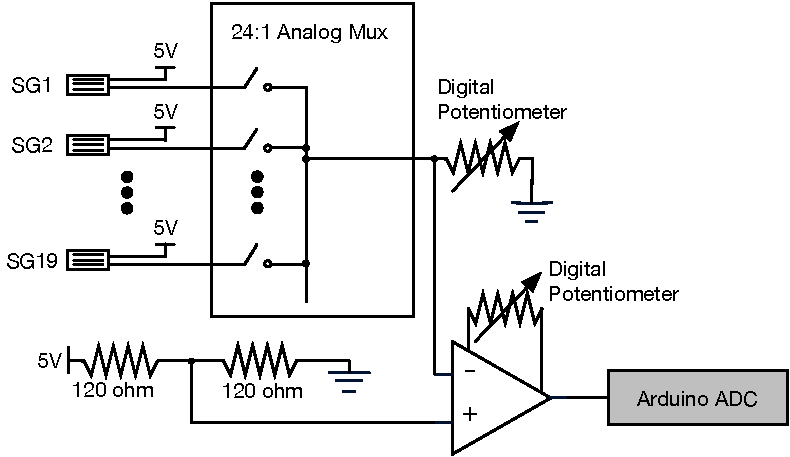
\includegraphics[width=1\columnwidth]{figures/CompleteDiagram_v2.pdf}
  \caption{The complete circuit diagram. Note that SG stands for strain gauge. The 24:1 analog multiplexer is practically made up of 3 analog multiplexers.}
  \label{fig:completeCircuitDiagram}
\end{figure}

\begin{figure}
 \begin{center}
  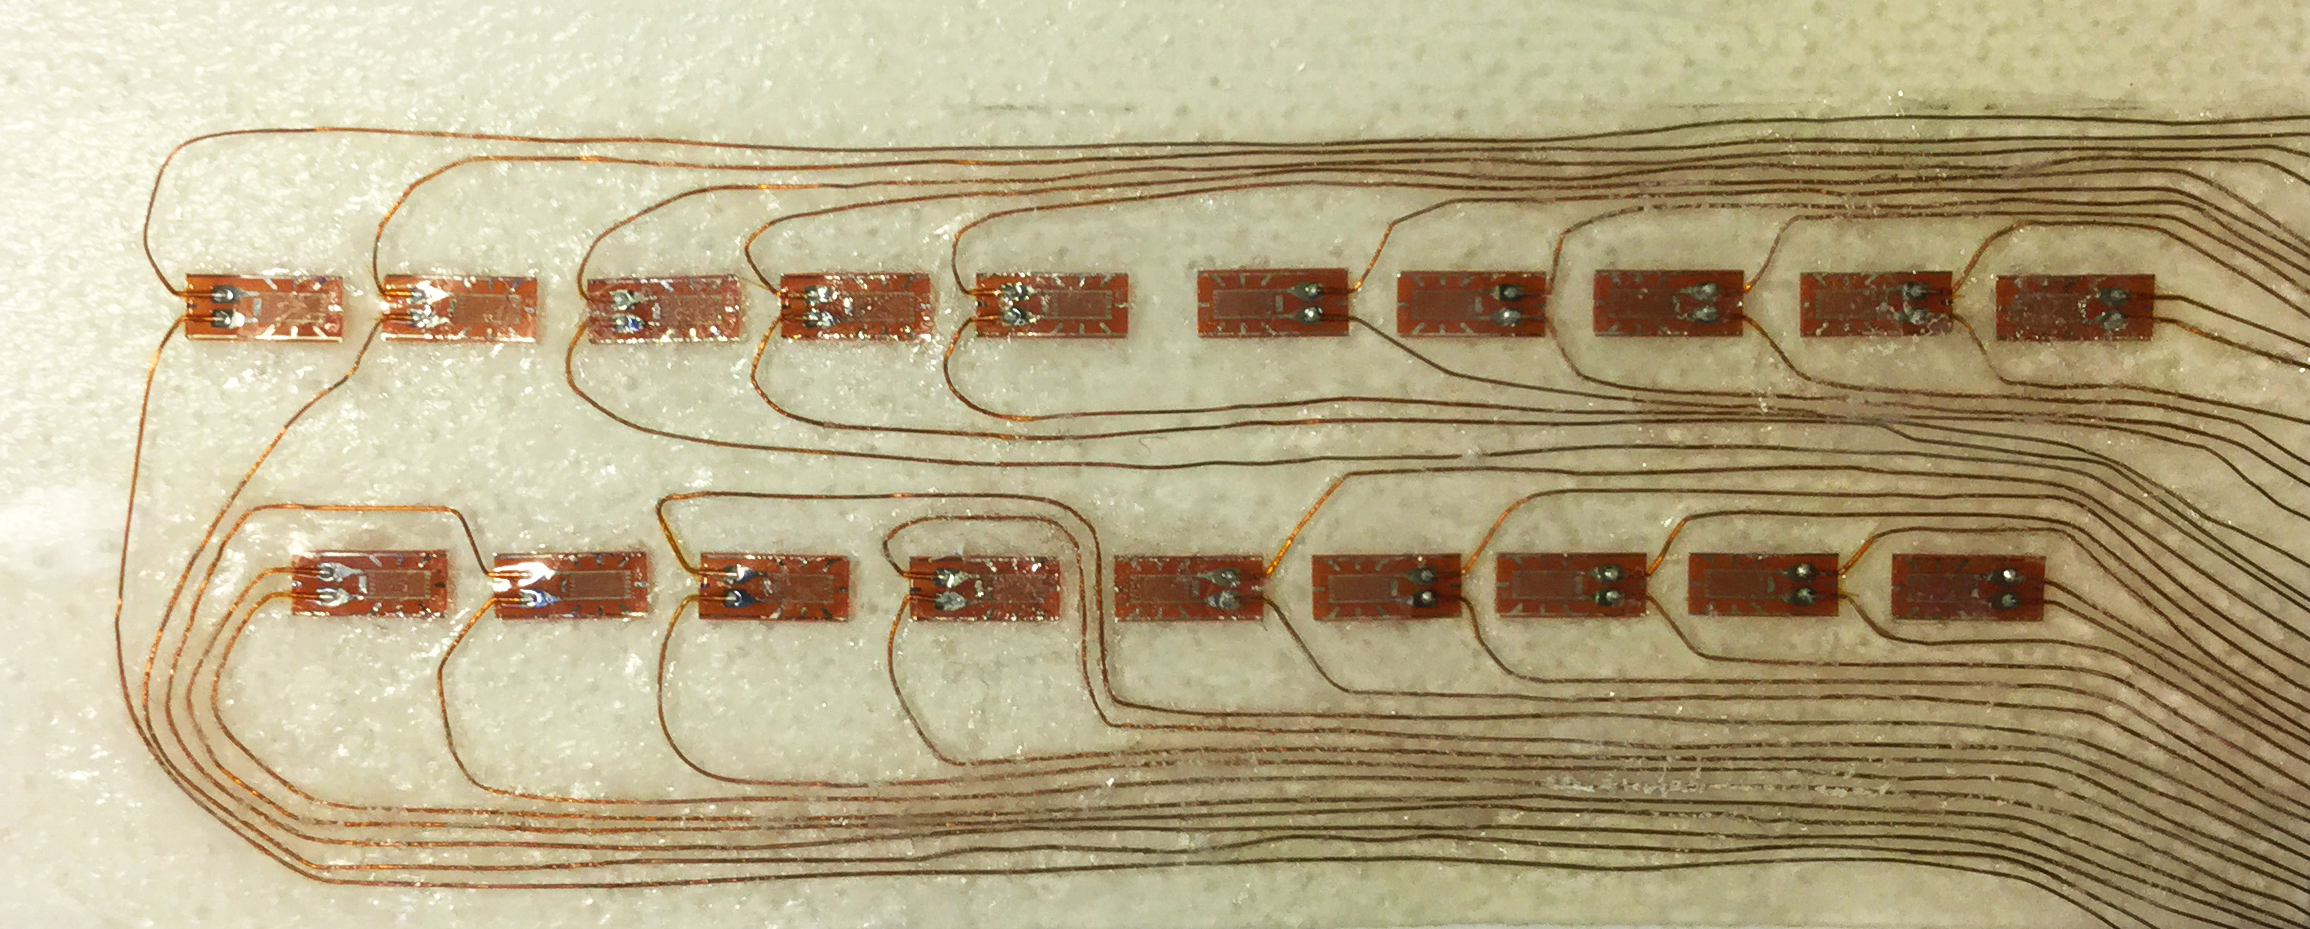
\includegraphics[width=1\columnwidth]{figures/tie.png}
  \caption{
    results
  }~\label{fig:tie}
  \end{center}
\end{figure}

The 19 sensors are read sequentially through the analog switches, so each sensor is electrically connected at a time. Once a sensor is active, the sensor became one of the 4 resistors on the Wheatstone bridge. The equivalent electric circuit is shown in \autoref{fig:equivalentCircuitDiagram}. Since the resistance of each sensor varies under no applied external force, a digital potentiometer in series with the connected sensor for calibration is also a resistor on the Wheatstone bridge. Another digital potentiometer serves the purpose of amplifier gain adjustment. In our prototype, the instrumental amplifier gain is set to be approximately 800 to 1000. Due to the dynamic response time of the amplifier, a 100-microsecond delay is added between each reading leading to a sampling rate of 526 Hz for our prototype.

\begin{figure}
  \begin{center}
  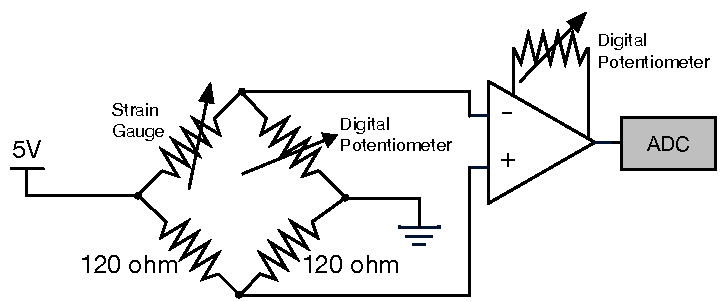
\includegraphics[width=1\columnwidth]{figures/EquivalentDiagram.pdf}
  \caption{The equivalent circuit diagram of an electrically connected strain gauge sensor.}
  \label{fig:equivalentCircuitDiagram}
  \end{center}
\end{figure}

\subsection{Machine Learning}

\section{EVALUATION: OPTIMAL SENSOR PLACEMENT}

The purpose of this evaluation was to investigate the accuracy of the different sensor placement ranging from back of the hand to wrist. 
The optimal sensor placement maximizes the performance of identifying hand gestures.
In addition, we provide some scientific visualizations of physical changes on the back of hand caused by gestures that are collected from all participants. These can enable us to understand, illustrate, and provide insight from collecting data. %by collecting data

\subsection{Study Design}
We recruited 10 participants (4 female, 8 right-handed) aged between 20 and 32 (mean: 23.2) to test 16 gestures, shown in \autoref{fig:gestureSet16}

\begin{figure}
  \begin{center}
  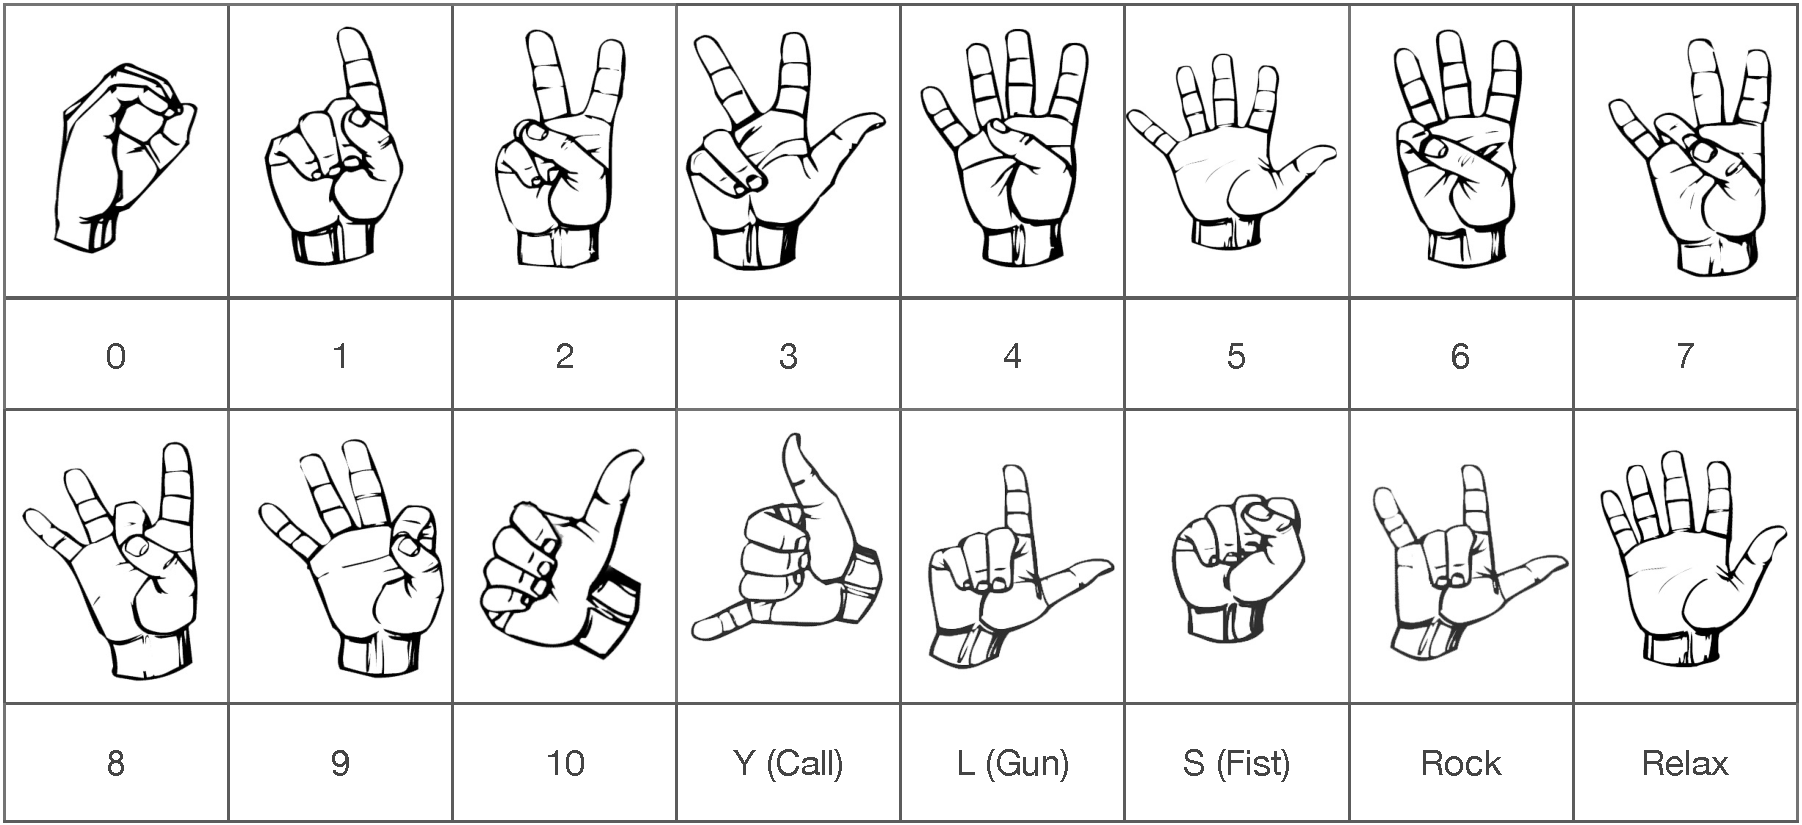
\includegraphics[width=1\columnwidth]{figures/gestureSet_16_v2.pdf}
  \caption{
    16 Gestures
  }\label{fig:gestureSet16}
  \end{center}
\end{figure}

We mainly picked this gesture set from American Sign Language (ASL), which is used as a primary means of communication for over one half million people in the United States [Mitchell et al. 2006]. 
In principle, there are 36 classes in the dataset. However, without considering the hand direction and movement, there are gestures that are notoriously difficult to classify between letters and digits due to their similarities.
For example, taking no account of rotation invariant method, “Z” “1” are too similar. 
Other examples are “2” against “V” and “K”, “H” against ”U“, ”I“ against ”J“ etc.
We properly excluded letters in ASL because the primary purpose of this study is to explore the influence of finger movements on back of the hand with various gesture.
Eventually, we choose digits from 1 to 10 in ASL and add other five daily life gestures (e.g. fist, call, rock etc) and one was hand in a relaxed position.

Figure X shows the study setup. The participants rested their right arm and wrist on the tilt platform and were seated on a chair whose height they could adjust to perform the tasks with ease. The monitor in front of the participants displayed instructions during the study.

\subsection{Procedure}
Initially, 8 rows (16 positions) across participants’ back of the hands were uniformly sampled and marked. The sampling scope ranged from the position of metacarpophalangeal joints (MCP, the knuckle between the hand and the finger) to the head of ulna (at the wrist).%see figure
The markers served as affixing targets for artificial skin composed of arrays of 19 strain gauges. 
Figure X illustrates the process using 19 strain gauges (2 rows each time) to gather information of hand movements.

We then affixed the artificial skin composed of arrays of strain gauges to these 8-row markers on the right hand for 4 rounds (2 rows each time). 
At each round, each participant performed each of 16 gestures randomly from on-screen instructions. Each gesture was trained 3 times; Each of them was sampled at 10 Hz in a duration of 2 seconds.

For the evaluation, each participant then performed the similar task as training sessions. Each gesture was done 7 times. The order of the gestures was randomly selected. The instructions for each specific gesture were displayed but without showing what the gesture was classified. 
Overall, the study took approximately 80 minutes per participants.

\subsection{Results}
Accuracy is defined as the number of correctly classified samples divided by the total number of samples. The accuracy due to chance was 20\%. In a 10-fold cross validation, the mean accuracy of the optimal sensor placement across all participants was 99.96\% (SD: ±2.7\%). Cross-validation represents the upper bound of accuracy. Also, we computed accuracy using the initial training data only, which reflects the real-time performance of the system. In this case, the accuracy was 91.17\% (SD: ±3.88\%). 

\begin{figure*}
 \begin{center}
  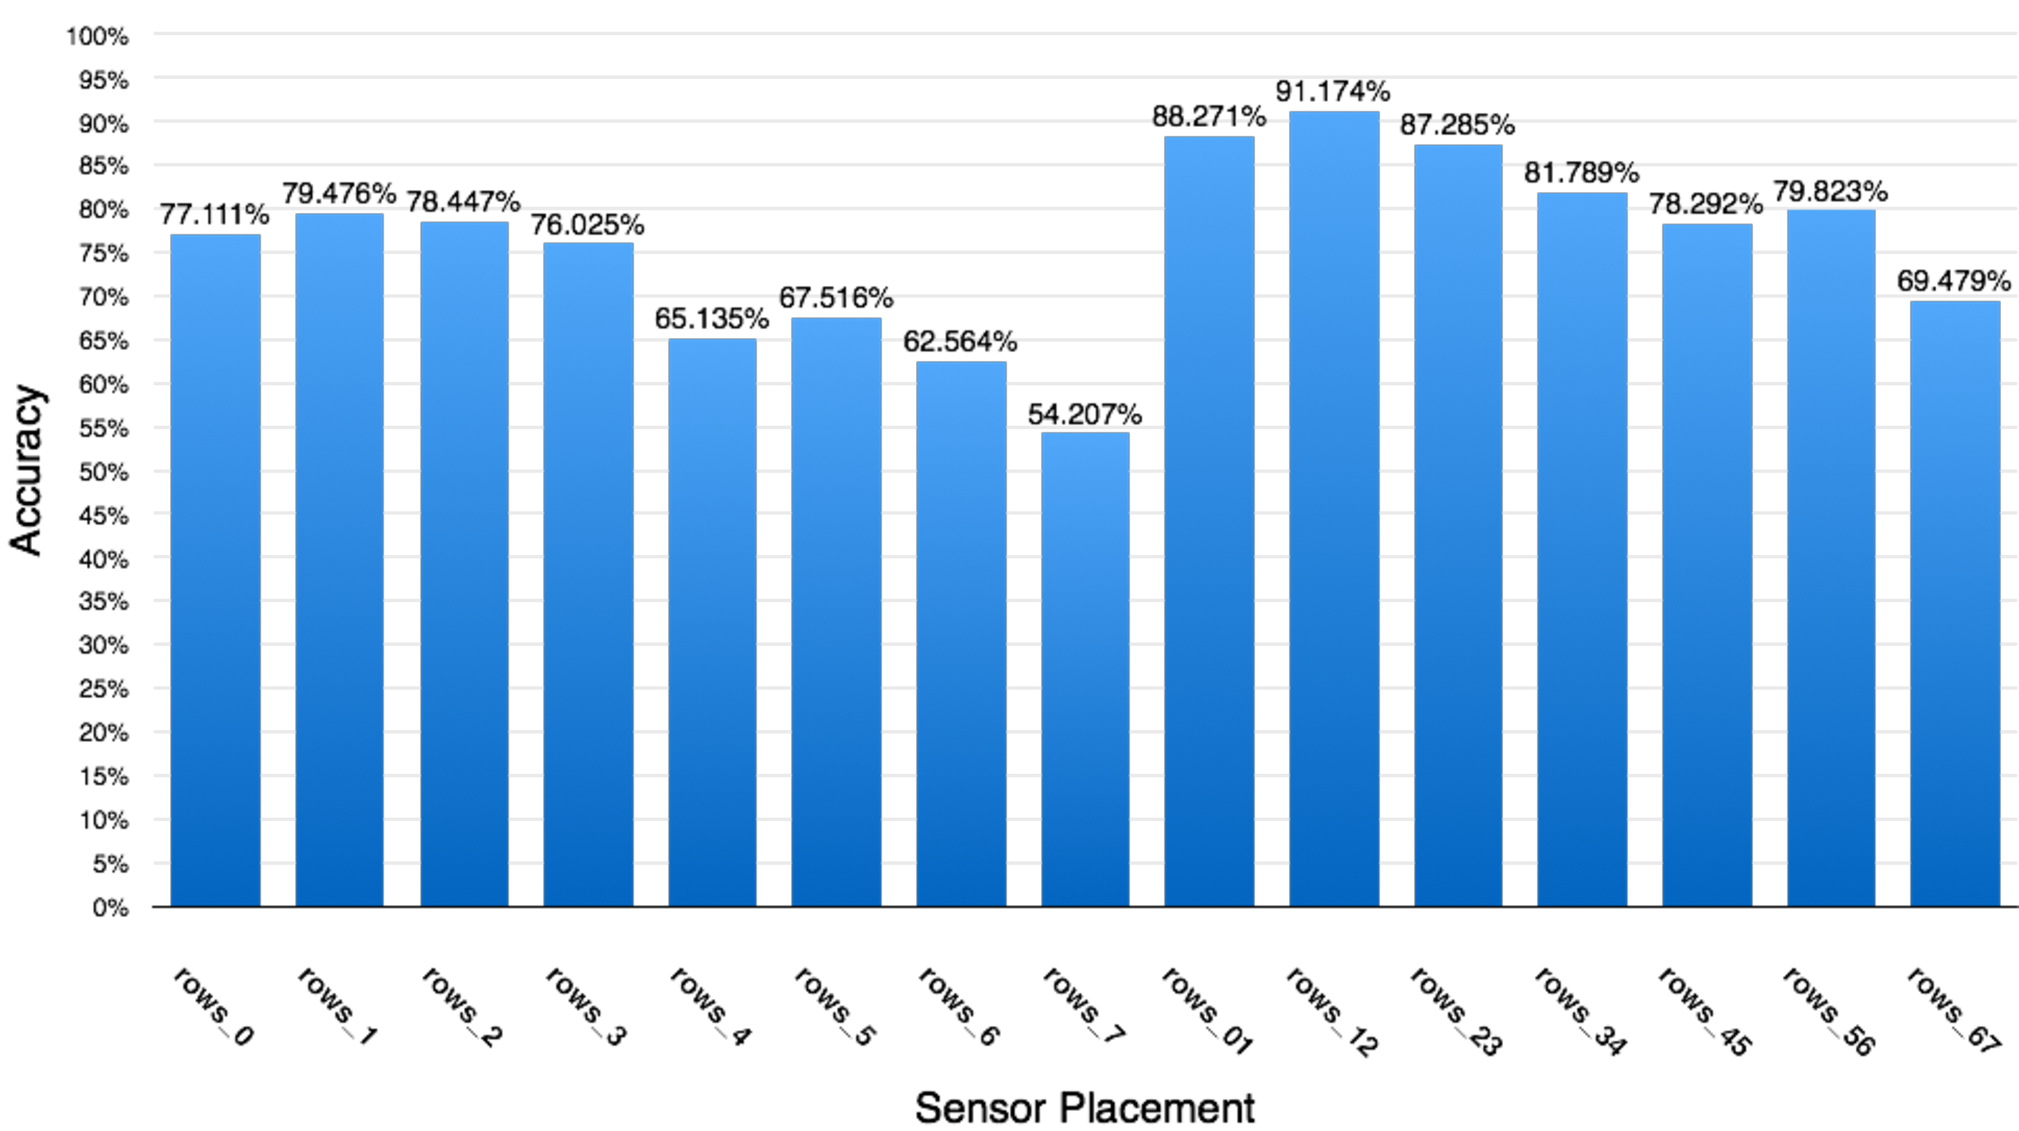
\includegraphics[width=2\columnwidth]{figures/accuracy16Gs.pdf}
  \caption{
    results
  }~\label{fig:accuracy16Gs}
  \end{center}
\end{figure*}

The results show that (1) the row12 had the highest accuracy rate, indicating the optimal sensor placement is not located closest to the finger joints but second to it. (2) The , indicating that.

\section{EXAMPLE APPLICATIONS}
Eight rows (Sixteen positions) across participants’ back of the hands were uniformly sampled and marked. The markers served as attaching targets for artificial skin composed of an array of strain gauges. Figure X illustrates the process using 19 strain gauges (two rows each time) to gather information of hand movements.

\section{DISCUSSION}
This template include a sample ACM copyright notice at the bottom.
\subsubsection{Sub-subsections}

Headings for sub-subsections should be in Helvetica or Arial 9-point
italic with initial letters capitalized.  Standard
\texttt{{\textbackslash}section}, \texttt{{\textbackslash}subsection},
and \texttt{{\textbackslash}subsubsection} commands will work fine in
this template.
%%%



% Use a numbered list of references at the end of the article, ordered
% alphabetically by first author, and referenced by numbers in
% brackets~\cite{ethics, Klemmer:2002:WSC:503376.503378,
%   Mather:2000:MUT, Zellweger:2001:FAO:504216.504224}. For papers from
% conference proceedings, include the title of the paper and an
% abbreviated name of the conference (e.g., for Interact 2003
% proceedings, use \textit{Proc. Interact 2003}). Do not include the
% location of the conference or the exact date; do include the page
% numbers if available. See the examples of citations at the end of this
% document. Within this template file, use the \texttt{References} style
% for the text of your citation.

% Your references should be published materials accessible to the
% public.  Internal technical reports may be cited only if they are
% easily accessible (i.e., you provide the address for obtaining the
% report within your citation) and may be obtained by any reader for a
% nominal fee.  Proprietary information may not be cited. Private
% communications should be acknowledged in the main text, not referenced
% (e.g., ``[Robertson, personal communication]'').

\begin{table}
  \centering
  \begin{tabular}{r c c}
    \toprule
    & \multicolumn{2}{c}{\small{\textbf{Caption}}} \\
    \cmidrule(r){2-3}
    {\small\textbf{Objects}}
    & {\small \textit{Pre-2002}}
    & {\small \textit{Current}} \\
    \midrule
    Tables & Above & Below \\
    Figures & Below & Below \\
    \bottomrule
  \end{tabular}
  \caption{Table captions should be placed below the table. We
    recommend table lines be 1 point, 25\% black. Minimize use of
    unnecessary table lines.}~\label{tab:table1}
\end{table}


\section{Conclusion}

It is important that you write for the SIGCHI audience. Please read
previous years’ proceedings to understand the writing style and
conventions that successful authors have used. It is particularly
important that you state clearly what you have done, not merely what
you plan to do, and explain how your work is different from previously
published work, i.e., the unique contribution that your work makes to
the field. Please consider what the reader will learn from your
submission, and how they will find your work useful. If you write with
these questions in mind, your work is more likely to be successful,
both in being accepted into the conference, and in influencing the
work of our field.

\section{Acknowledgments}

Sample text: We thank all the volunteers, and all publications support
and staff, who wrote and provided helpful comments on previous
versions of this document. Authors 1, 2, and 3 gratefully acknowledge
the grant from NSF (\#1234--2012--ABC). \textit{This whole paragraph is
  just an example.}

% Balancing columns in a ref list is a bit of a pain because you
% either use a hack like flushend or balance, or manually insert
% a column break.  http://www.tex.ac.uk/cgi-bin/texfaq2html?label=balance
% multicols doesn't work because we're already in two-column mode,
% and flushend isn't awesome, so I choose balance.  See this
% for more info: http://cs.brown.edu/system/software/latex/doc/balance.pdf
%
% Note that in a perfect world balance wants to be in the first
% column of the last page.
%
% If balance doesn't work for you, you can remove that and
% hard-code a column break into the bbl file right before you
% submit:
%
% http://stackoverflow.com/questions/2149854/how-to-manually-equalize-columns-
% in-an-ieee-paper-if-using-bibtex
%
% Or, just remove \balance and give up on balancing the last page.
%
\balance{}

\section{References Format}


% REFERENCES FORMAT
% References must be the same font size as other body text.
\bibliographystyle{SIGCHI-Reference-Format}
\bibliography{sample}

\end{document}

%%% Local Variables:
%%% mode: latex
%%% TeX-master: t
%%% End:
